\begin{figure}[htbp]
\section*{ SLC32A1}
\centering
\begin{subfigure}[b]{0.95\textwidth}
\centering
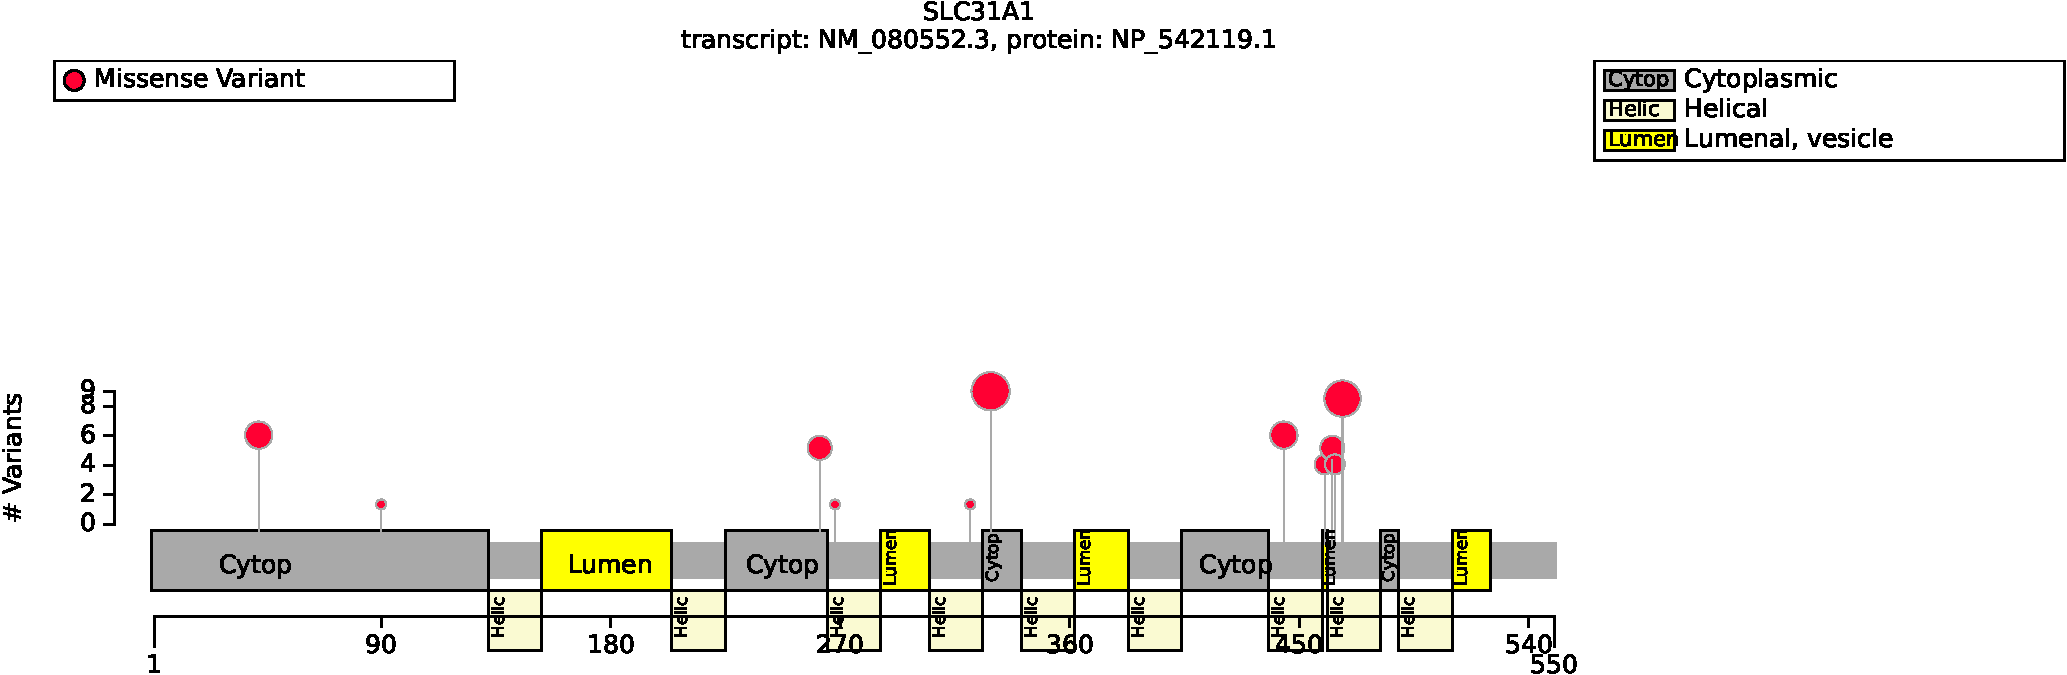
\includegraphics[width=\textwidth]{ img/SLC32A1_protein_diagram.pdf} 
\captionsetup{justification=raggedright,singlelinecheck=false}
\caption{Distribution of variants in SLC32A1}
\end{subfigure}

\vspace{2em}

\begin{subfigure}[b]{0.95\textwidth}
\centering
\resizebox{\textwidth}{!}{
\begin{tabular}{llllrr}
\toprule
Genotype (A) & Genotype (B) & total tests performed & significant results\\
\midrule
N term & other & 11 & 0\\
p.Met330Thr & Other variant & 11 & 0\\
FEMALE & MALE & 11 & 0\\
\bottomrule
\end{tabular}
}
\captionsetup{justification=raggedright,singlelinecheck=false}
\caption{             Fisher Exact Test performed to compare HPO annotation frequency with respect to genotypes. }
\end{subfigure}

\vspace{2em}

\caption{ The cohort comprised 38 individuals (19 females, 19 males). A total of 44 HPO terms were used to annotate the cohort. Disease diagnoses: Generalized epilepsy with febrile seizures plus, type 12 (OMIM:620755) (34 individuals), Developmental and epileptic encephalopathy 114 (OMIM:620774) (4 individuals). No significant correlation identified. A total of 12 unique variant alleles were found in \textit{SLC32A1} (transcript: \texttt{NM\_080552.3}, protein id: \texttt{NP\_542119.1}).}
\end{figure}
